\documentclass[a4paper, 11pt]{article}
\usepackage[utf8]{inputenc} % Change according your file encoding
\usepackage{graphicx}
\usepackage{url}
\usepackage[margin=1in]{geometry}
\usepackage{caption}
\usepackage{subcaption}
\usepackage{float}

\usepackage[catalan,english]{babel}


%% Estil de Paràgraf
\setlength{\parskip}{4mm}
\setlength{\parindent}{0mm}

%% Estil lletra
\renewcommand{\familydefault}{\sfdefault}
 
%opening
\title{Seminar Report: Mutty}
\author{Martín Garcia \and Ferran Arau}
\date{\today{}}

\begin{document}

\maketitle

\section{Introducció}

% Introduce in a couple of sentences the seminar and the main topic related to
% distributed systems it covers.

El seminari té com objectiu implementar un sistema d'exclusió mutua entre
diferents nodes d'un sistema distribuït. 

Cada node disposa d'una regió crítica associada. En aquest cas la regió crítica
és un codi artificial que ''dorm'' durant un temps quan és executat, s'anomena
\textit{worker}. No pot haver més d'un node executant el seu \textit{worker}
simultàniament. 

Donat l'escenàri exposat cal implementar en erlang el sistema de comunicacions
entre els processos per tal de garantir l'exclusió mutua, així com els possibles
deadlocks. 

La tècnica utilitzada per dur a terme la implementació és l'exposada pel
document \textit{An optimal Algorithm for mutual Exclusion in Computer Networks}
publicat per en Glen Ricart i l’Ashok K. Agrawala.

\section{Feina de laboratori}

A continuació es presenten les tres implementacions del sistema de locks. Es
mostren les diferències entre el codi original i el de producció mitjançant les
eines de ''history'' que proporciona el repositori utilitzat. 

Es pot consultar el codi d'aquesta sessió a
\url{https://github.com/magarcia/SDX/tree/master/S2}

\subsection{Lock1}

La primera implementació és donada per l'assignatura i no ha estat necessari
modificar-la. No obstant, s'han fet les proves recomanades. S'ha pogut apreciar
els diversos comportaments del sistema modificant els paràmetres de
\texttt{Sleep} i \texttt{Work}.

A continuació es mostren les estadístiques generades a partir de les proves.

\subsubsection{Prova amb Sleep 2000, Work 2000}

\begin{figure}[H]
	\centering
    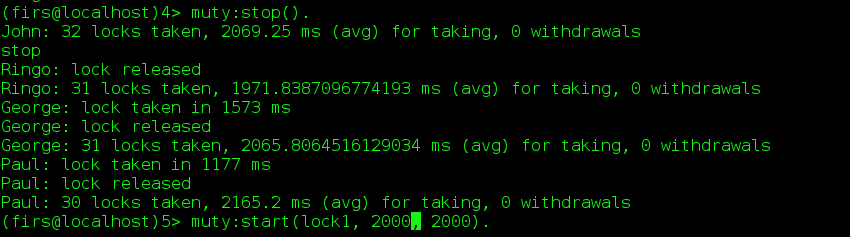
\includegraphics[width=1.0\textwidth]{figures/2000-2000lock1}
    \caption{Sleep 2000, Work 2000 \label{fig:2000-2000lock1}}    
\end{figure}
% (muty@localhost)7> muty:stop().
% John: 51 locks taken, 1968.1960784313726 ms (avg) for taking, 0 withdrawals
% Paul: 46 locks taken, 2053.6739130434785 ms (avg) for taking, 0 withdrawals
% stop
% Ringo: lock released
% Ringo: 48 locks taken, 1956.6458333333333 ms (avg) for taking, 0 withdrawals
% George: lock taken in 3954 ms
% George: lock released
% George: 50 locks taken, 1999.16 ms (avg) for taking, 0 withdrawals
% (muty@localhost)8>


Es pot veure que l'execució és l'esperada. El \texttt{withdrawal} és de 8
segons, tal i com està per defecte. En la figure~\ref{fig:2000-2000lock1} es pot
veure que aquest valor està a zero per tots els clients. Per tant, no hi ha cap
d'ells que s'hagi vist obligat a rellançar la petició d'accés a regió crítica.

Donat que el temps de sleep és ''gran'' no es forcen locks. 

\subsubsection{Prova amb Sleep 20, Work 16000}

\begin{figure}[H]
	\centering
    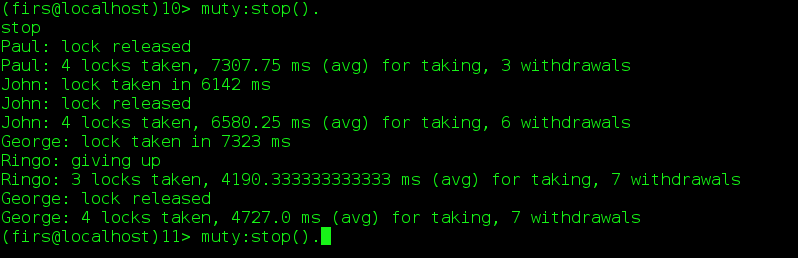
\includegraphics[width=1.0\textwidth]{figures/20-16000lock1}
    \caption{Sleep 20, Work 16000 \label{fig:20-16000lock1}}    
\end{figure}
% (muty@localhost)3> muty:stop().
% stop
% Paul: lock released
% Paul: 12 locks taken, 6528.666666666667 ms (avg) for taking, 25 withdrawals
% John: lock taken in 5156 ms
% John: lock released
% John: 18 locks taken, 6120.111111111111 ms (avg) for taking, 22 withdrawals
% George: lock taken in 6222 ms
% Ringo: giving up
% Ringo: 12 locks taken, 5258.25 ms (avg) for taking, 31 withdrawals
% George: lock released
% George: 15 locks taken, 5781.2 ms (avg) for taking, 24 withdrawals
% (muty@localhost)4>

En aquest experiment s'ha forçat que els workers sol·licitin accés a regió
crítica de manera molt freqüent, en proporció a la finestra de temps que un
worker necessita per executar-se.  
Es pot apreciar a la figure~\ref{fig:20-16000lock1} que el rendiment del sistema
baixa notòriament. El temps mig d'espera augmenta molt amb aquesta prova degut a
que hi ha molts intents d'accés a regió crítica no resolts. El paràmetre
\texttt{withdrawal} ha augmentat perquè hi ha molts processos que es veuen
forçats a fer el timeout i sol·licitar accés a regió crítica de nou.

\subsubsection{Prova amb Sleep 20, Work 20}

\begin{figure}[H]
	\centering
    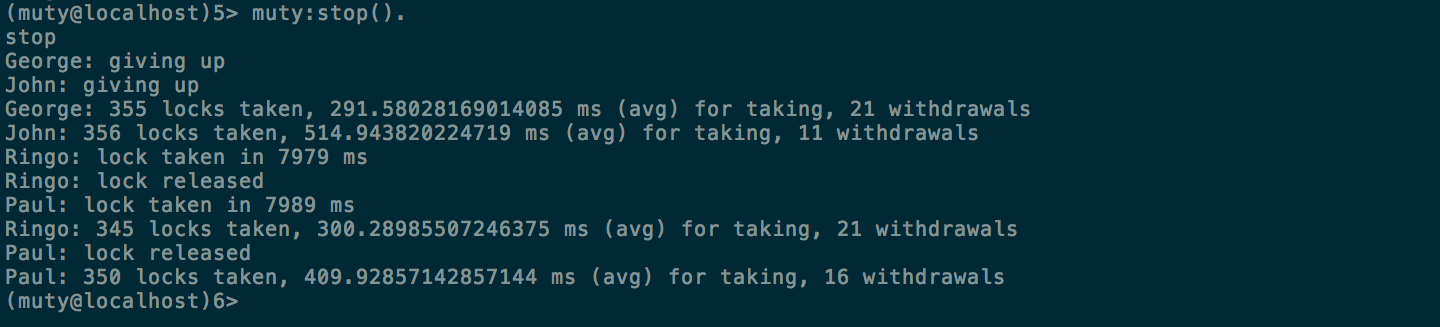
\includegraphics[width=1.0\textwidth]{figures/20-20lock1}
    \caption{Sleep 20, Work 20 \label{fig:20-20lock1}}    
\end{figure}
% (muty@localhost)5> muty:stop().
% stop
% George: giving up
% John: giving up
% George: 355 locks taken, 291.58028169014085 ms (avg) for taking, 21 withdrawals
% John: 356 locks taken, 514.943820224719 ms (avg) for taking, 11 withdrawals
% Ringo: lock taken in 7979 ms
% Ringo: lock released
% Paul: lock taken in 7989 ms
% Ringo: 345 locks taken, 300.28985507246375 ms (avg) for taking, 21 withdrawals
% Paul: lock released
% Paul: 350 locks taken, 409.92857142857144 ms (avg) for taking, 16 withdrawals
% (muty@localhost)6>

Per concloure les proves fetes sobre la implementació \textit{lock1} s'ha
estudiat el comportament amb valors de \texttt{Sleep} i \texttt{Work}
''petits''. En aquest experiment s'ha pogut veure que el sistema distribuit
pateix un \emph{deadlock}. Tots els nodes executen la sol·licitud d'accés a les regions
crítiques respectivament al mateix temps. Això provoca que tots vegin que la
seva sol·licitud és la prioritària i per tant no validin la resta de requests.

\subsection{Lock2}

La segona implementació consisteix en solucionar els possibles \emph{deadlocks}.
Per fer-ho s'ha utilitzat un sistema de prioritats a partir d'identificadors
lògics de node. El node més petit és el que té prioritat, alhora d'entrar a la
regió crítica, en cas d'empat.

\subsubsection{Prova amb Sleep 2000, Work 2000}

\begin{figure}[H]
    \centering
    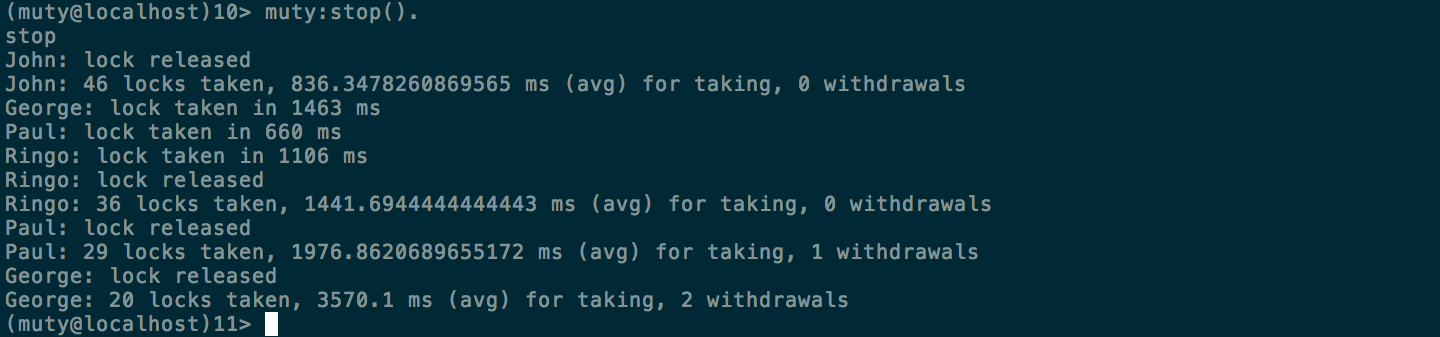
\includegraphics[width=1.0\textwidth]{figures/2000-2000lock2}
    \caption{Sleep 2000, Work 2000 \label{fig:2000-2000lock2}}    
\end{figure}
% (muty@localhost)10> muty:stop().
% stop
% John: lock released
% John: 46 locks taken, 836.3478260869565 ms (avg) for taking, 0 withdrawals
% George: lock taken in 1463 ms
% Paul: lock taken in 660 ms
% Ringo: lock taken in 1106 ms
% Ringo: lock released
% Ringo: 36 locks taken, 1441.6944444444443 ms (avg) for taking, 0 withdrawals
% Paul: lock released
% Paul: 29 locks taken, 1976.8620689655172 ms (avg) for taking, 1 withdrawals
% George: lock released
% George: 20 locks taken, 3570.1 ms (avg) for taking, 2 withdrawals
% (muty@localhost)11>

\subsubsection{Prova amb Sleep 20, Work 16000}

\begin{figure}[H]
    \centering
    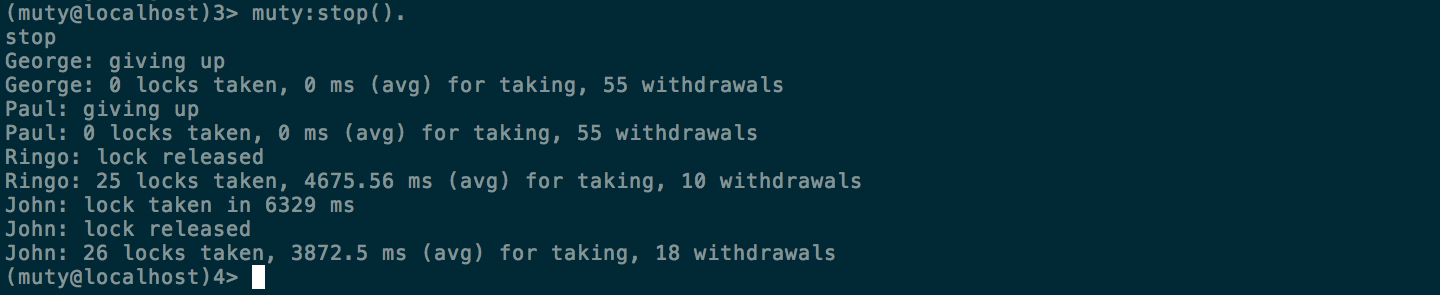
\includegraphics[width=1.0\textwidth]{figures/20-16000lock2}
    \caption{Sleep 20, Work 16000 \label{fig:20-16000lock2}}    
\end{figure}
% (muty@localhost)3> muty:stop().
% stop
% George: giving up
% George: 0 locks taken, 0 ms (avg) for taking, 55 withdrawals
% Paul: giving up
% Paul: 0 locks taken, 0 ms (avg) for taking, 55 withdrawals
% Ringo: lock released
% Ringo: 25 locks taken, 4675.56 ms (avg) for taking, 10 withdrawals
% John: lock taken in 6329 ms
% John: lock released
% John: 26 locks taken, 3872.5 ms (avg) for taking, 18 withdrawals
% (muty@localhost)4>

\subsubsection{Prova amb Sleep 20, Work 20}

\begin{figure}[H]
    \centering
    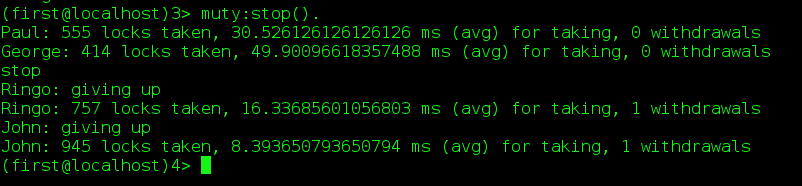
\includegraphics[width=1.0\textwidth]{figures/20-20lock2}
    \caption{Sleep 20, Work 20 \label{fig:20-20lock2}}    
\end{figure}
% (muty@localhost)5> muty:stop().
% stop
% John: 2863 locks taken, 8.308767027593433 ms (avg) for taking, 0 withdrawals
% Paul: lock released
% Paul: 1675 locks taken, 30.918805970149254 ms (avg) for taking, 0 withdrawals
% George: lock released
% George: 1253 locks taken, 48.65203511572226 ms (avg) for taking, 0 withdrawals
% Ringo: giving up
% Ringo: 2300 locks taken, 15.862173913043478 ms (avg) for taking, 1 withdrawals
% (muty@localhost)6>

\subsection{Lock3}

\section{Preguntes directes}

% Try to answer all the open questions in the documentation. When possible, do
% experiments to support your answers.

\section{Opinió personal}


\end{document}

